\section{Лапароскопічний погляд на хірургічну анатомію печінки}

Лапароскопічна хірургія має відмінності у візуалізації порівняно із відкритою хірургією, які пов'язані із відображенням плоскої, спотворенної заломленням світла при проходженні крізь оптичну частину лапароскопа проекції тривимірного зображення на екран. Такі відмінності зумовлюють особливий вигляд анатомічних структур та затруднюють їх ідентифікацію відносно звичних орієнтирів. Розуміння принципів виникнення таких особливостей є основою для безпечного виконання \acrshort{llr}. У цьому підрозділі ми розглянемо сучасні погляди на анатомічну будову печінки та особливості її лапароскопічної візуалізації.

\subsection{Сучасна номенклатура хірургічної анатомії печінки}

Резекційна хірургія печінки в теперішньому вигляді не була б можливою без детального уявлення про її внутішню анатомічну будову. Сучасні знання про анатомію печінки базуються на работах Healey J., Schroy P. і Couinaud С., які розробили принципи сегментарного поділу печінки. В класифікації Couinaud С., печінка поділяється на ліву та праву напів-печінку, кожна з яких в свою чергу ділеться на медіальний та латеральний сектори по ходу лівої та правої печінкових вен \cite{COUINAUD1954}. Кожен з секторів, окрім лівого латерального далі поділяється на два сегменти. Першим сегментом (Sg I) печінки є каудальна доля, яка має автономне кровопостачання. Враховуючи каудальну долю загальна кількість сегментів по Couinaud складає 8 (у більш пізній версії класифікації автор виділив хвостатий відросток Sg I у окремий 9-й сегмент) і вони мають нумерацію по ходу годинної стрілки за анологією з районами Парижу. Кожен сегмент за Couinaud - це ділянка паренхіми печінки, яка має автономне кровопостачання та жовчовідтік за рахунок гілок глісонів третього порядку. 

\begin{figure}[h]
\caption{Сегментація печінки за C.Couinaud.}

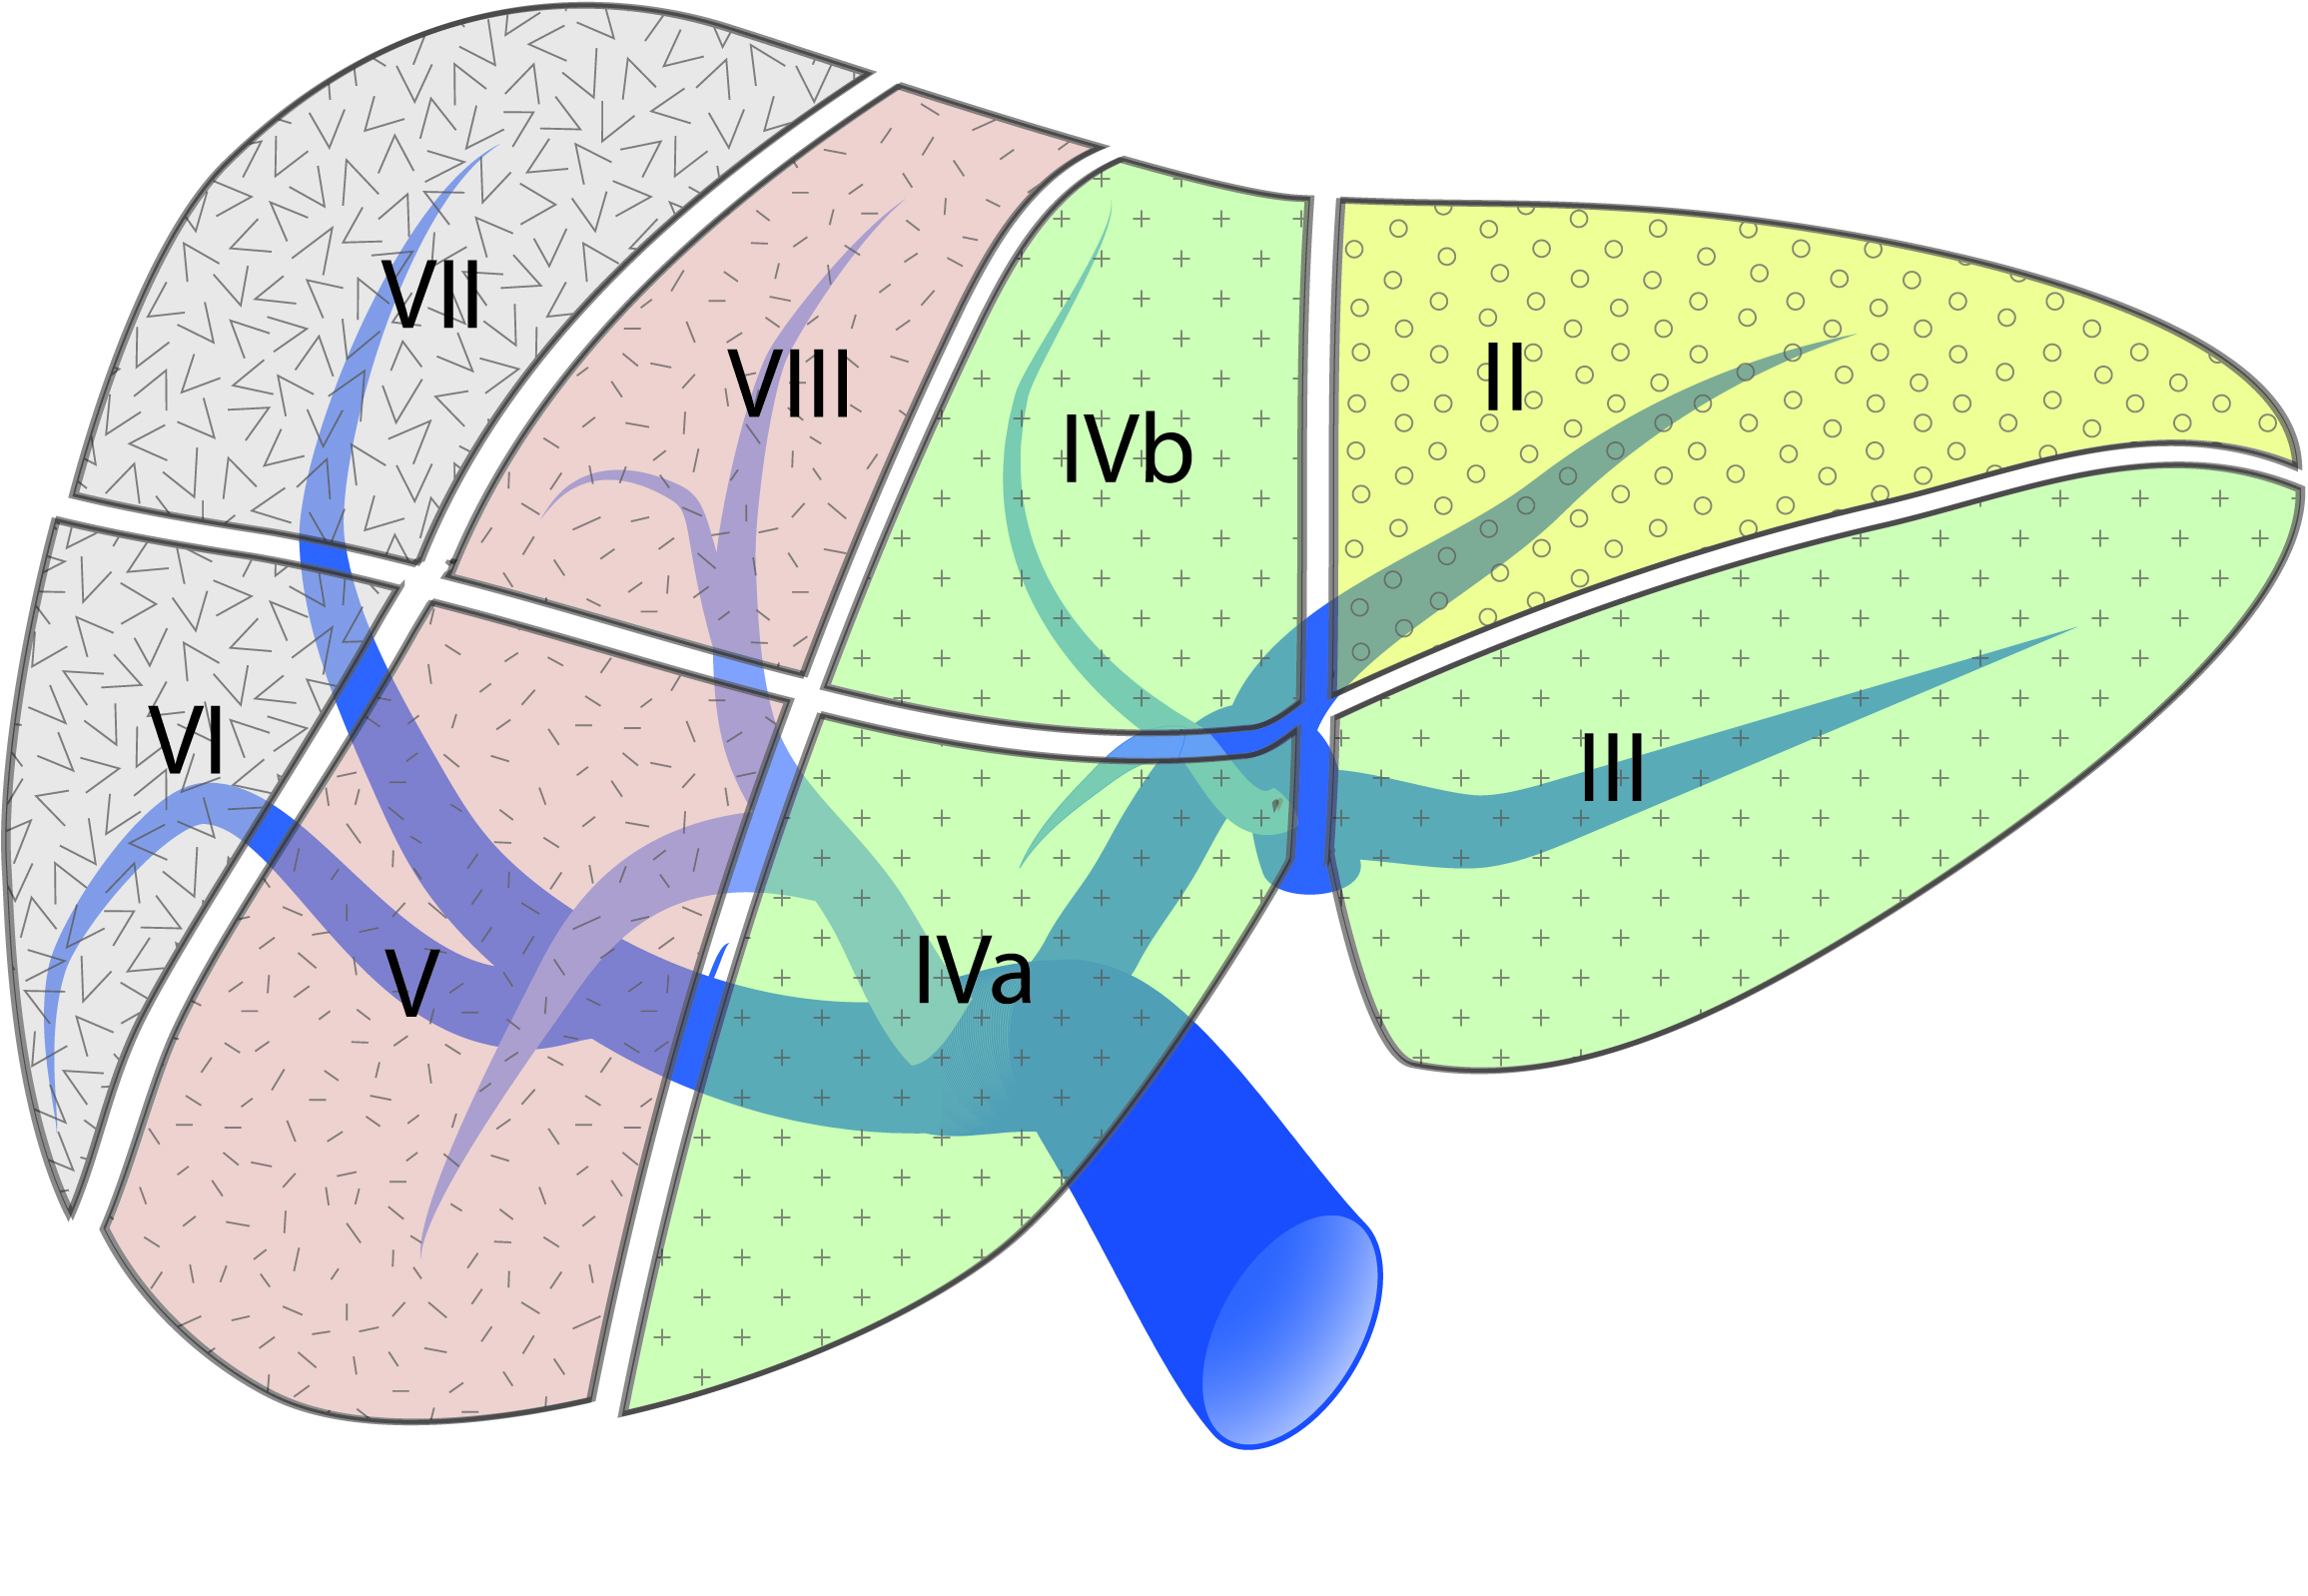
\includegraphics[width=0.9\textwidth]{Illustrations/Chapter_01/Couinaud.jpg}
\label{fig:Couinaud}

\medskip
\small
С. Сектори позначені окремими візерунками, сегменти позначені окремими контурами та римськими цифрами. Каудальна доля на малюнку не відображена. Синім кольором зображена ворітна вена.

\end{figure}

Класифікація Healey J. та Schroy P. використовує подібний принцип поділу, але на відміну від класифікації Couinaud поділяє печінку на ліву та праву долі, що діляться на сегменти (аналог секторів за Couinaud), які в свою чергу діляться на ділянки (аналог сегментів за Couinaud) \cite{HEALEY1953}. Принципово в цих двох класифікаціях відрізняється принцип поділу лівої долі печінки, яку Couinaud поділяє на сектори за ходом ворітної вени (до медіального сектору віднесено Sg 3, 4 а до латерального -  Sg 2), а Healey на сегменти за ходом жовчних шляхів та печінковї артерії (до медіального сегменту віднесено Sg 4 а до латерального - Sg 2,3).  

\begin{figure}[h]
\caption{Сегментація печінки за Healey J. та Schroy P.}

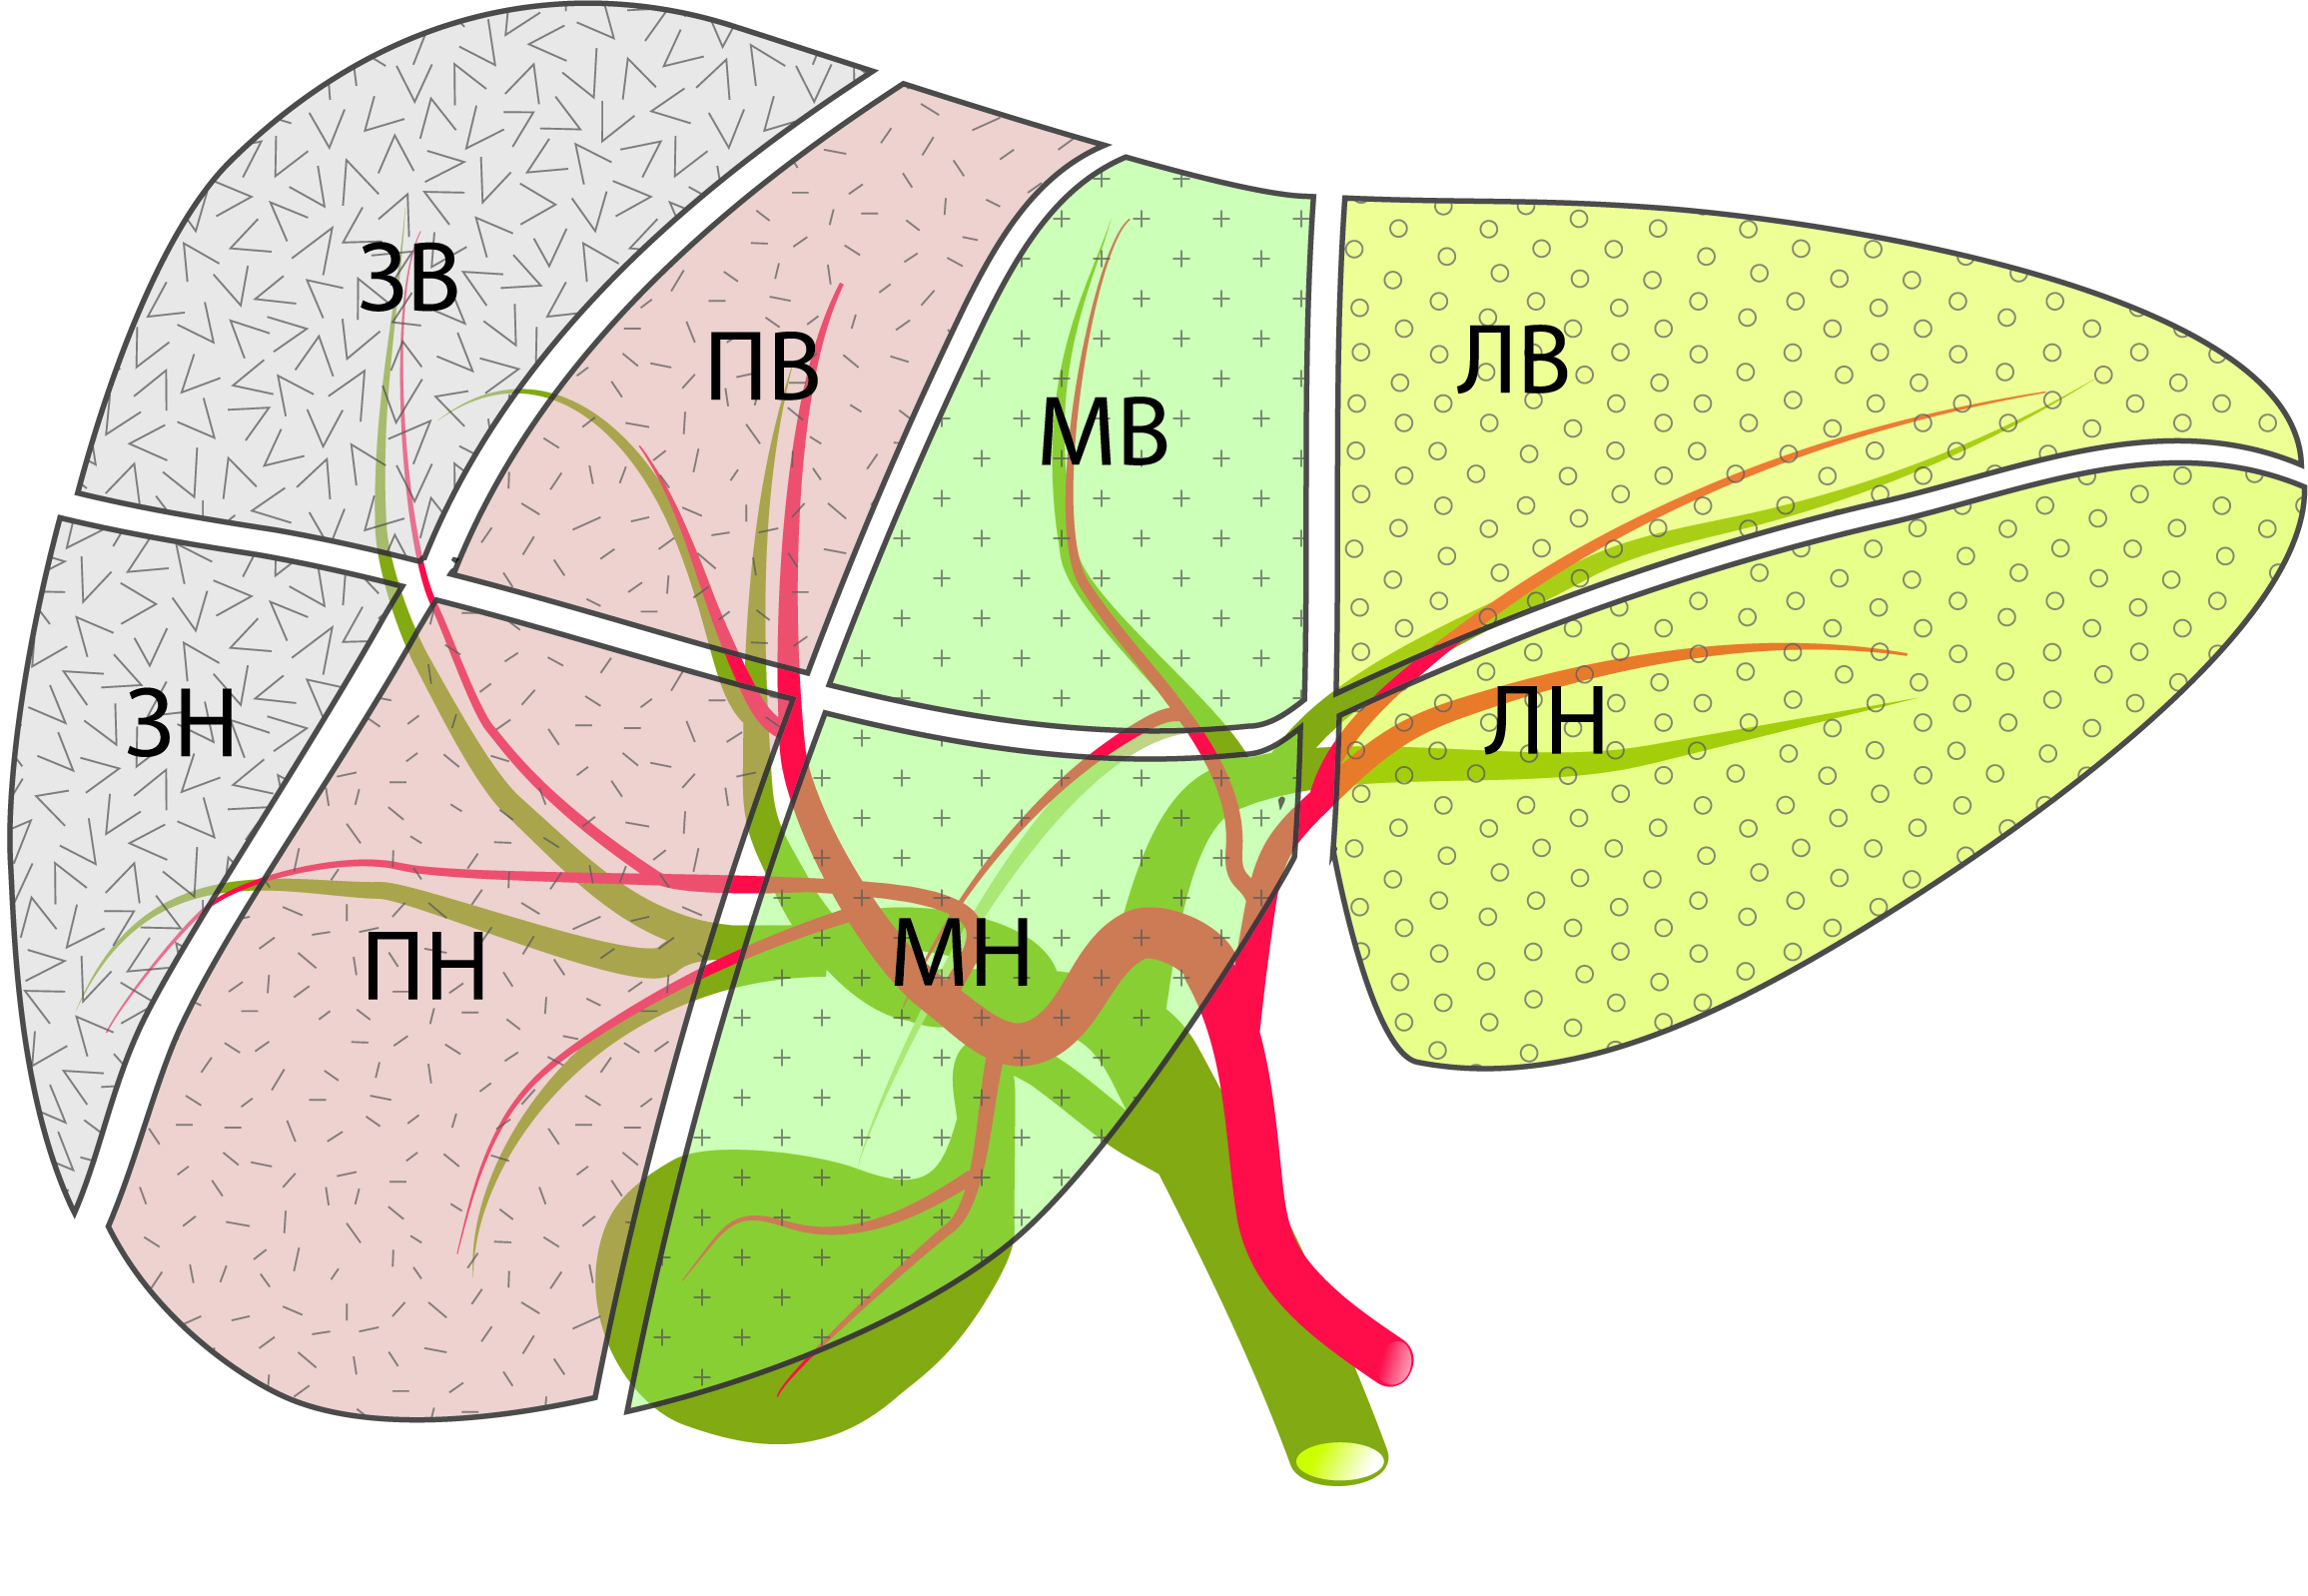
\includegraphics[width=0.9\textwidth]{Illustrations/Chapter_01/Healey.jpg}
\label{fig:Healey}

\medskip
\small
Сегменти позначені окремими візерунками, ділянки позначені окремими контурами скороченнями: ЛВ - латеральня верхня, ЛН - латеральна нижня, МВ - медіальна верхня, МН - медіальна нижня, ПВ - передня верхня, ПН - передня нижня, ЗВ - задня верхня, ЗН - задня нижня ділянка. Зеленим та червоним кольором зображені жовчні протоки та печінкова артерія відповідно.
\end{figure}

Так, як обидві класифікації мають широке розповсюдження в світі, з метою стандартизації на погоджувальній конференції в Брісбані у 2000 році Міжнародною Гепатопанкреатобіліарною Асоціацією було запропоновано універсальну номенклатуру для визначення анатомічних областей та видів резекцій печінки \cite{Pang2000}. Брисбанська класифікація побудована на основі класифікації Couinaud із заміною терміну "сектор" на "секція", за виключенням будови лівої долі, де Sg 2,3 віднесені до лівої латеральної секції. Згідно цієї класифікації таким анатомічним зонам, як напів-печінка (доля), секція та сегмент відповідають операції гемігепатектомія, секцієектомія та сегментектомія. Для уникнення термінологічних розбіжностей у цьому виданні ми будемо користуватись виключно номенклатурними термінами відповідно Брісбанській класифікації 2000 року.

\begin{figure}[h]
\caption{Брісбанська классифікація 2000 року номенклатури резекцій печінки}
\centering
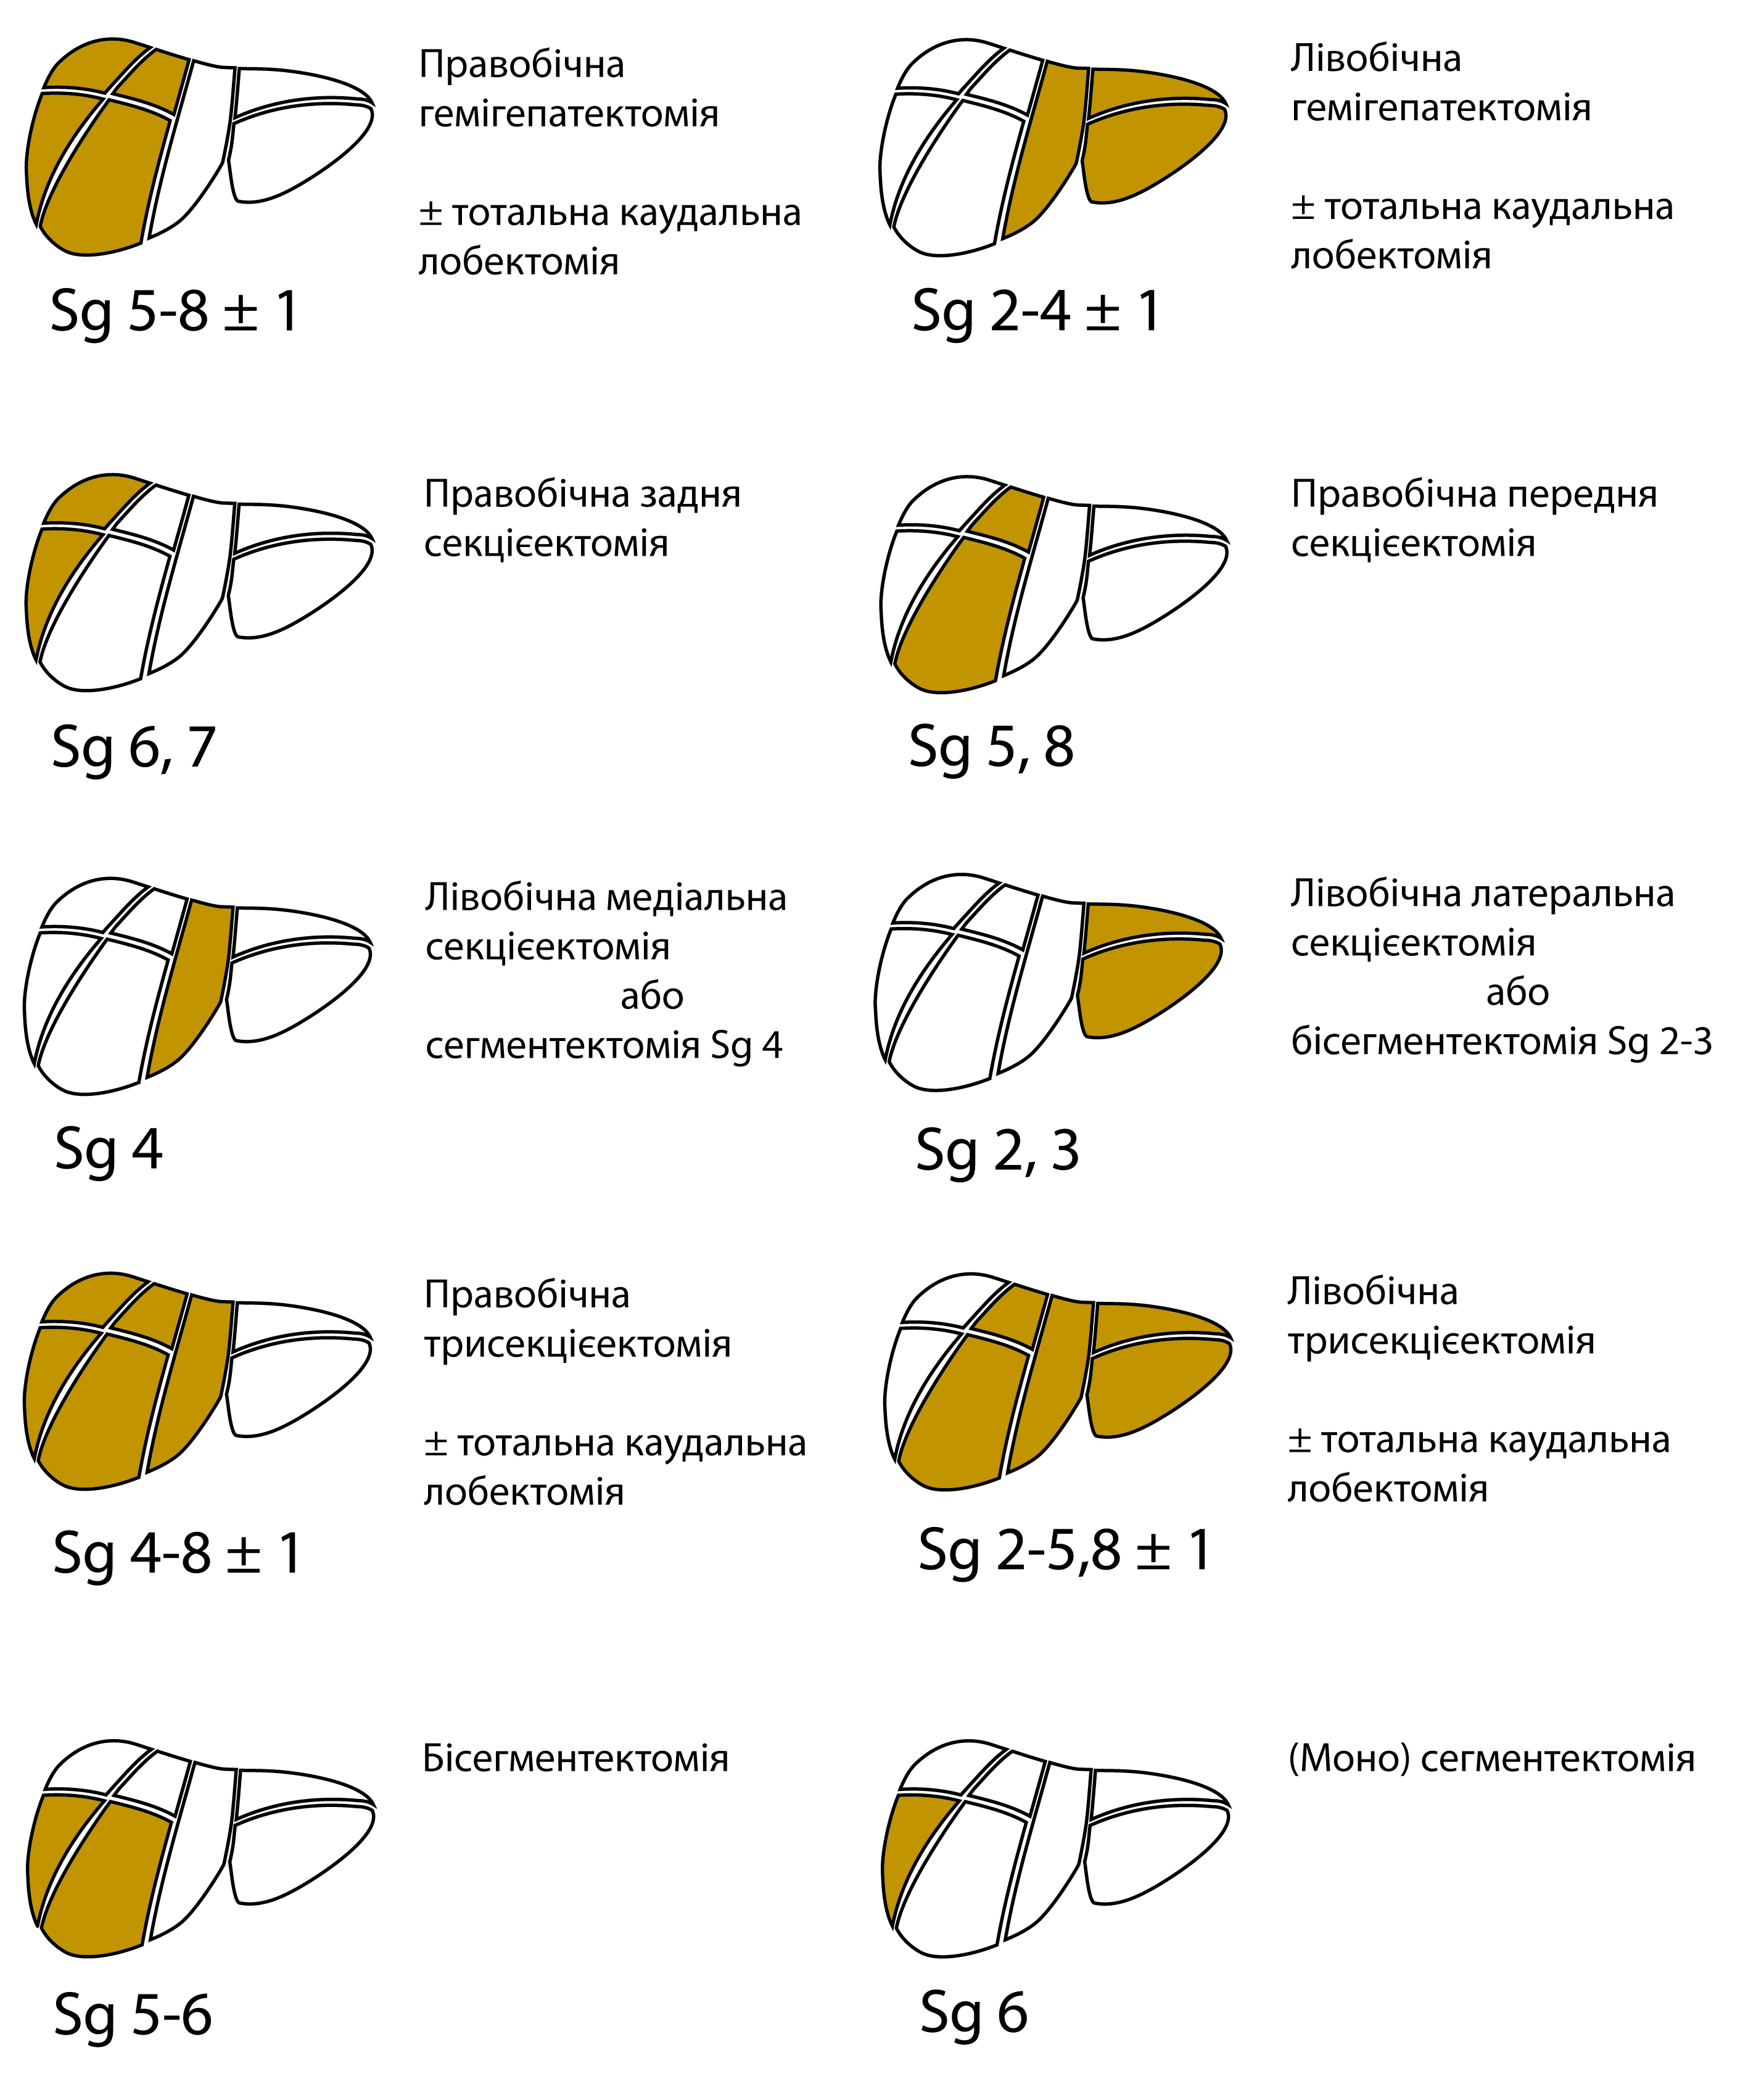
\includegraphics[width=0.9\textwidth]{Illustrations/Chapter_01/Brisbane.jpg}
\label{fig:Brisbane}
\end{figure}

\subsection{Лапароскопічна візуалізація зовнішніх орієнтирів}

На геометрію лапароскопічного зображення впливають кут огляду, кут напрямку зору та відстань до об'єкту. Скошена оптика (із кутом напрямку зору 30 та 45 градусів) дозволяє зробити огляд з різних боків, проте має більший ступінь спотворення зображення. Окрім того обмежений робочий простір, створений карбоксиперитонеумом, робить утрудненою візуалізацію цілого органу.

\subsubsection{Зв'язковий апарат}

Печінка вкрита очеревиною зі всіх боків, окрім невеликої частини  де очеревина переходить на діафрагму та формує коронарну зв'язку, яка далі переходить в ліву та праву трикутні зв'язки які разом утворюють її фіксуючий апарат. Серповидна зв'язка йде сагітально по серединній лінії від пупка та містить круглу зв'язку в свому вільному краї. Кругла зв'язка прямує до умбілікальної фіссури по вісцеральній поверхні лівої долі печінки, де входить в печінку та закінчується облітерованою частиною умбілікальної порції лівої ворітної вени. 

Серповидна зв'язка є чітким лапароскопічним орієнтиром, що відмежовує ліву латеральну секцію від інших сегментів печінки. Ліва трикутна зв'язка повністю доступна огляду по задньому краю Sg 2 печінки. Для візуалізації нижнього краю правої трикутної зв'язки необхідно підняти праву долю печінки. Верхній край правої трикутної зв'язки майже не доступний візуалізації без попередньої мобілізації її нижнього краю та коронарної зв'язки. 

\begin{figure}[h]
\caption{Лапароскопічний вигляд зовнішніх орієнтирів печінки}

\includegraphics[width=0.9\textwidth]{Illustrations/Chapter_01/External landmarks_Ligaments.png}
\label{fig:External_landmarks_Ligaments}

\small
а) Серповидна та кругла зв'язки б) Коронарна зв'язка в) Ліва трикутна зв'язка г) Нижній край правої трикутної зв'язки
\end{figure}



\subsubsection{Структури печінково-дванадцятиперсної зв'язки}

В складі печінково-дванадцятиперсної зв'язки (\acrshort{pdl}) в печінку входять ворітна вена, печінкова артерія, гілки блукаючого нерва, а виходять жовчні та лімфатичні протоки. Структури \acrshort{pdl} покриті жировою та сполучною тканиною і шаром очеревини, яка переходить в малий сальник по лівому краю зв'язки. Пряма лапароскопічна візуалізація структур \acrshort{pdl} без диссекції можлива лише частково, як правило у пацієнтів з малою кількістю інтраабдомінальної жирової тканини. Зовнішніми орієнтирами є шийка жовчного міхура, отвір Вінслоу та малий сальник. Після холецистектомії сають доступними до візуалізації проекції правих переднього та заднього глісонів та глісону каудального відростку Sg 1. 

\begin{figure}[h]
\caption{Проекція структур печінково-дванадцятиперсної зв'язки}

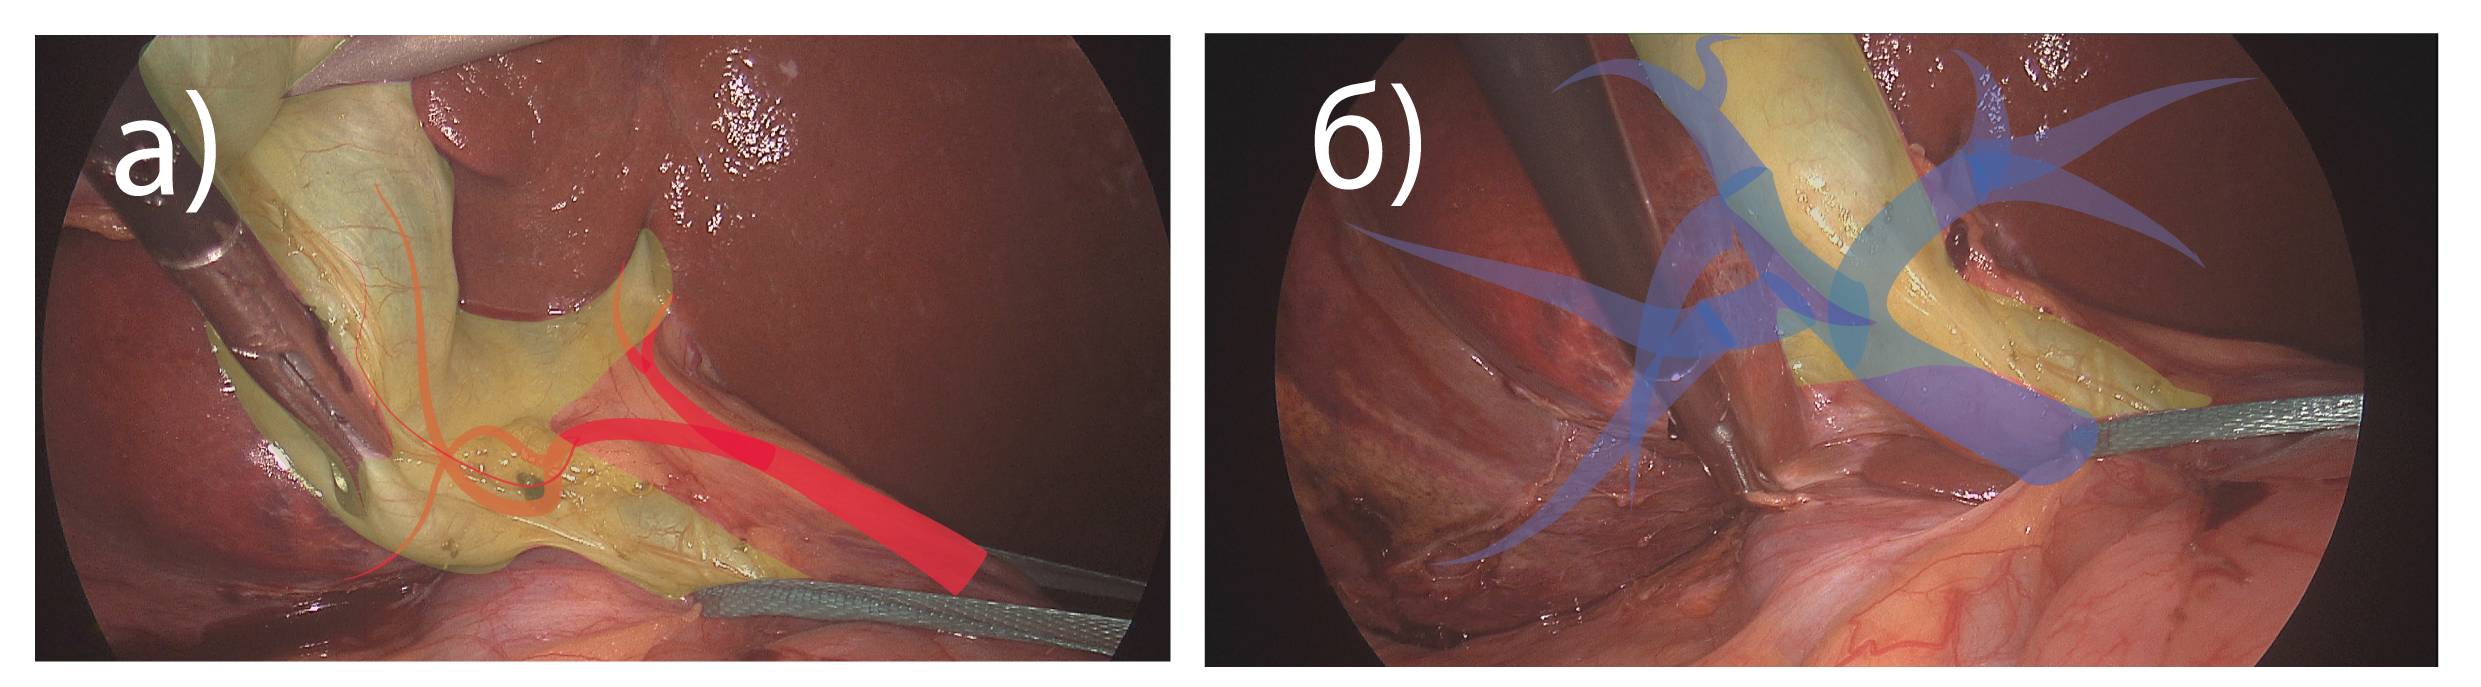
\includegraphics[width=0.9\textwidth]{Illustrations/Chapter_01/External landmarks_PDL.png}
\label{fig:External_landmarks_PDL}

\small
а) Проекція гілок печінкової артерії в товщі \acrshort{pdl} б) Проекція ствола та гілок ворітної вени (жовтим позначені жовчні шляхи)
\end{figure}


\subsection{Капсула Лаенека та концепція «вхідних воріт» для глісонового підходу}

Вперше описана Laennec в 1802 р. власна капсула печінки є тонкою мембраною, яка лежить субсерозно та на відміну від очеревини покриває цілий орган. Пізніше Couinaud була сформована концепція Глісонового плато - потовщеної фіброзної пластини, яка покриває судинно секреторні структури в складі Глісонових ніжок. Плато умовно ділять на три частини - хіларне, умбілікальне та міхурове, які переходять одне в інше. Також на основі гістологічних досліджень він довів, що капсула Лаенека не продовжується на Глісонові ніжки в складі хіларного плато, а йде окремим шаром вздовж усіх глісонових структур та печінкових вен, що входять в паренхіму печінки.

За сучасними уявленнями капсула Лаенека йде паралельно до глісонових структур, але в деякіх ділянках не прилягає до них щільно. Ця особливсість дає можливість безпечного хірургічного підходу до позапечінкового виділення Глісонових структур під час \acrshort{alr}, тому простір в місцях нещільного прилягання капсули Лаенека до глісонових гілок має назву "вхідних воріт" \cite{Sugioka2017}. Всього виділяють шість вхідних воріт для визначення яких є чотири анатомічних орієнтира - Аранцієва протока, умбілікальне плато, міхурове плато та Глісонова ніжка каудального відростка. Межею I воріт є каудальний кінець Аранцієвої протоки, II воріт - з'єднання між круглою зв'язкою та умбілікальним плато, III воріт - правий край лівого дольового глісону (Sg 2-4), IV воріт - лівий край правого переднього глісону, V воріт - біфуркація правих сегментарних глісонів, а VI воріт - простір між краєм заднього глісону та глісоном каудального відростку. 

\begin{figure}[h]
\caption{Вхідні "ворота" капсули Лаенека}

\includegraphics[width=0.9\textwidth]{Illustrations/Chapter_01/Gates.jpg}
\label{fig:Gates}

\small
Ворота позначено червоними ділянками та римськими цифрами I-VI.
\end{figure}


Диссекція в цих анатомічних ділянках та послідовне з'єднання між собою сусідніх воріт дозволяє виконати позапечінкову ізоляцію будь якого глісону з метою наступного виконання анатомічної резекції. Усі вхідні ворота легко доступні для лапароскопичноъ візуалізації: ворота I - III безпосередньо, а ворота IV - VI після попередньої холецистектомії (мал №)

\subsection{Анатомічна будова Sg I печінки}

Перший сегмент печінки або каудальна доля це центродорзально розташована ділянка паренхіми, яка має незалежне кровопостачання та жовчевідтік. Анатомічно вона обмежена наступними структурами: по задньому краю запечінковим сегментом \acrshort{ivc}, по нижньому краю воротами печінки, по верхньому - устям правої та загальним устям лівої та серединної печінкових вен, по пердньому та правому краю - тканиною Sg 4-8, а по лівому має зовнішню поверхню, вкриту капсулою (Спігелєва доля), яка пролабує до малого сальника та обмежена Аранцієвим протоком. Відповідно до класифікації Kumon M. \cite{Kumon2017}, каудальна доля поділяється на три частини: 1) Спігелєва порція (доля),  2) Паракавальна порція, 3) Порція каудального відростка. Для прямої лапароскопічної візуалізації  доступна лише частина каудального відростка та спігелєва доля після розсічення малого сальника.

Каудальна доля має власні портальні гілки, які йдуть від біфуркації ворітної вени в дорзальному напрямку. Аналогічно до портальних гілок, каудальна доля має власні артеріальні гілки від лівої та правої печінкових артерій та жовчні протоки, що дренуються в області конфлюенся лівого та правого дольових жовчних протоків. Спігєлева доля та порція каудального відростка мають по одній власній печінковій вені а паракавальна порція - декілька коротких печінкових вен, які дренуються безпосередньо в \acrshort{ivc}. 

\begin{figure}[h]
\caption{Анатомія Sg1 печінки}
\centering
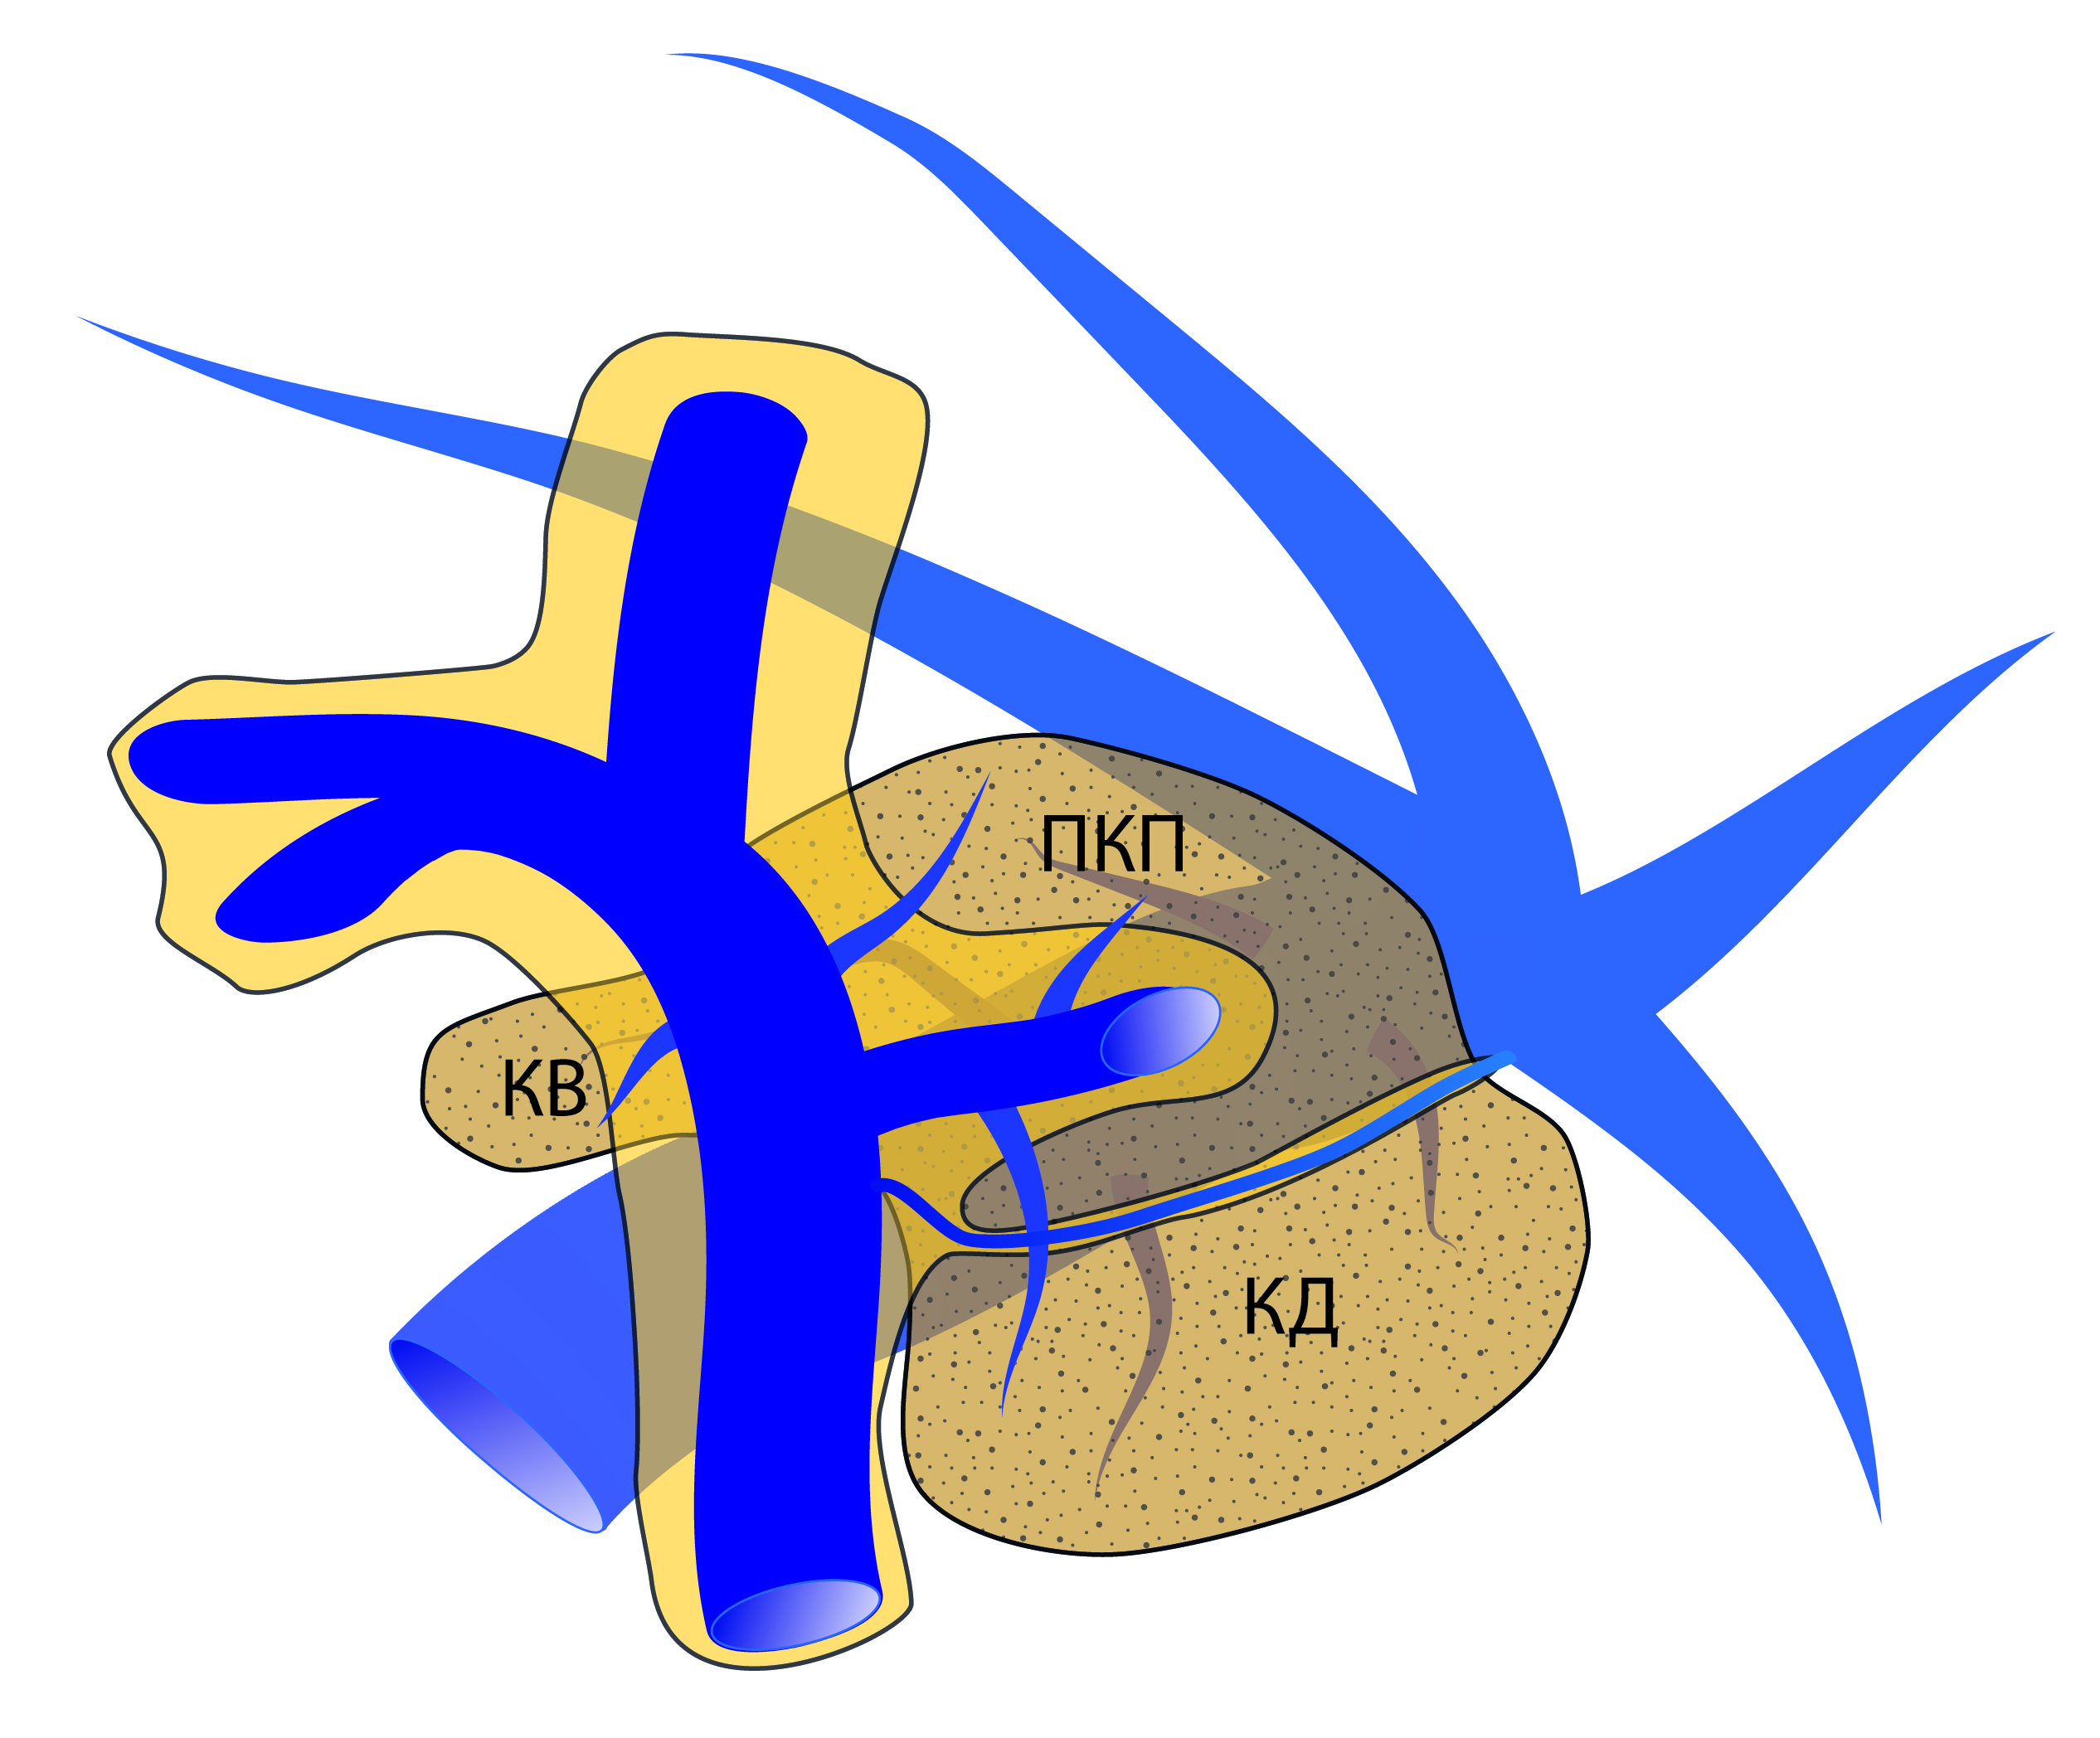
\includegraphics[width=0.9\textwidth]{Illustrations/Chapter_01/Sg1.jpg}
\label{fig:Sg1}
\end{figure}

\subsubsection{Нижня порожниста вена та печінкові вени}

Запечінковий сегмент \acrshort{ivc} інтимно прилягає до Sg 1 печінки звідки в нього дренуються короткі печінкові вени та обмежений згори окремим устям правої та загальним устям лівої та серединної печінкових вен. Для повної лапароскопічної візуалізації \acrshort{ivc} необхідна мобілізація правої трикутної та кронарної зв'язки та тракція правої долі печінки ліворуч.